
\section{Introdução}




\noindent \begin{minipage}[c]{0.6\textwidth}
  \vspace {1cm}
\par Na diciplina de programação e desenvolvimento de banco de dados é apresentado as discentes a linguagem \textbf{SQL} \textit{Structured Query Language},

\end{minipage}
\begin{minipage}[c]{0.4\textwidth}
  \captionof{figure}{Placeholder}
  
\includegraphics[width=\textwidth]{figure/placeholder.jpg}
  	\label{fig:place}
    {\fontsize{10pt}{\baselineskip}\selectfont
    Fonte: \citeonline{linux:2023}
  }

\end{minipage}


\section{Desenvolvimento}
\par Para implementação deta aula prática formam estabelecidos algumas regras informadas no roteiro \href{https://github.com/OgliariNatan/database_and_data_development/blob/main/aula%20pr%C3%A1tica.pdf}{da aula prática,} sendo a atividade proposta:
\begin{itemize}
  \item Criar uma estrutura de um banco de dados com a linguagem \textbf{SQL} por meio de uma entidade-relacionamento pré-definido.
  \item Inserir dados no banco de dados criado.
  \item Consultar os dados armazenados por meio da criação de uma vião \textit{View}.
  \item Criar um relatório no final da atividade.
\end{itemize}
\par Na atividade proposta o relatório dispõe de alguns procedimentos para a realização da atividade. Sugere a criação de uma base de dados de uma loja com o nome do banco de \textbf{Loja}, com a utilizazão de definições de dados \textbf{DDL} da linguagem SQL, e respeítando o modelo definido no \textbf{DER}, porposto pela atividade conforme figura \ref{fig:DER}.

\begin{figure}[!h]
  \caption{Diagrama entidade relacionamento}
  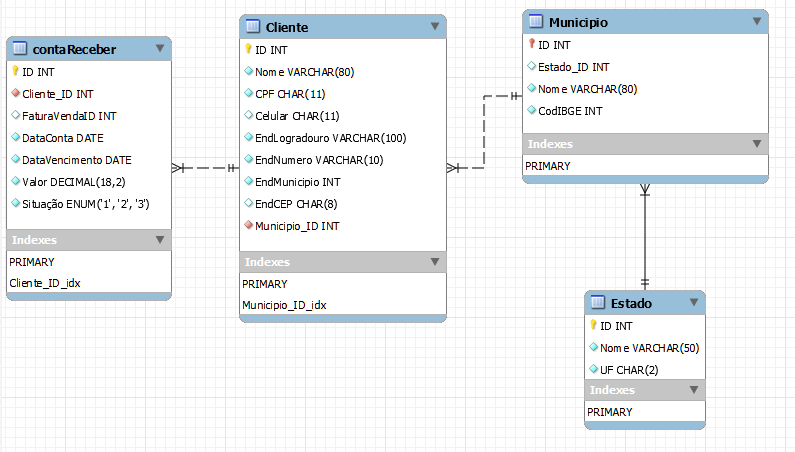
\includegraphics[width=\textwidth]{figure/diagram_EER.png}
  \label{fig:DER}
  {\fontsize{10pt}{\baselineskip}\selectfont
  Fonte: O autor.}
\end{figure}



\section{Método}

\lstinputlisting[caption={inserir.sql}, label={cod:inserir}]{inserir.sql}



\section{Conclusões}


  %$X \xLongleftarrow[\text{NATAN}]{\text{OGLIARI}} Y $ %COM TEXTO
	% $\uparrow$ %Seta para Cima
	%$\overleftarrow{NATAN}$
